\documentclass[letterpaper,10pt]{article}
% use UTF8 encoding
\usepackage[utf8]{inputenc}
% use KoTeX package for Korean 
\usepackage[english]{babel}
\usepackage{multirow}
\usepackage{array}
\usepackage[dvipsnames]{xcolor}
\usepackage{kotex}
\usepackage{adjustbox}
\usepackage{tabularx} % extra features for tabular environment
\usepackage{amsmath}  % improve math presentation
\usepackage{amssymb}
\usepackage{graphicx} % takes care of graphic including machinery
\usepackage[margin=1in,letterpaper]{geometry} % decreases margins
\usepackage{cite} % takes care of citations
\usepackage[final]{hyperref} % adds hyper links inside the generated pdf file
\usepackage{minted}
\hypersetup{
	colorlinks=true,       % false: boxed links; true: colored links
	linkcolor=blue,        % color of internal links
	citecolor=blue,        % color of links to bibliography
	filecolor=magenta,     % color of file links
	urlcolor=blue         
}
\usepackage{blindtext}
%++++++++++++++++++++++++++++++++++++++++


\setlength{\parskip}{1.0em}
\renewcommand{\baselinestretch}{1.25}
\begin{document}
	
	\title{3. Multi-Layer perceptron}
	\author{2019920017 컴퓨터과학부 김정현}
	\date{2021/10/19까지}
	\maketitle
	
	\section{구현 방법 소개}
	
	\subsection{MLP의 각 구성 요소를 모듈화}
	
	이전에 제출한 과제(2. $n$차원 입력의 Perceptron Learning)에서 하나의 Single-Layer Perceptron을 구현하기 위해 각 구성 요소를 별도의 Class로 구현하였다. 이번 과제에서 MLP(Multi-Layer Perceptron)을 구현하는 것에도 이와 유사한 패러다임을 차용하였다. MLP에서 입력 벡터에 가중치 행렬을 곱하여 출력 벡터를 계산하는 완전 연결 계층(Fully Connected)은 물론 Sigmoid와 같은 활성화 함수(Activation Function) 까지 공통된 추상 클래스(Module)을 상속 받도록 구현한다면 MLP를 구현하는 것은 이렇게 만든 Module들을 적절히 조립하는 것으로 단순화된다.
	
	본 과제에서 구현된 Fully-Connected 계층과 활성화 함수, 오차 함수는 Figure \ref{fig:module}, \ref{fig:error} 과 같이 Module, Error 추상 클래스를 상속 받도록 구현하였다.
	
	\begin{figure}
		\centering
		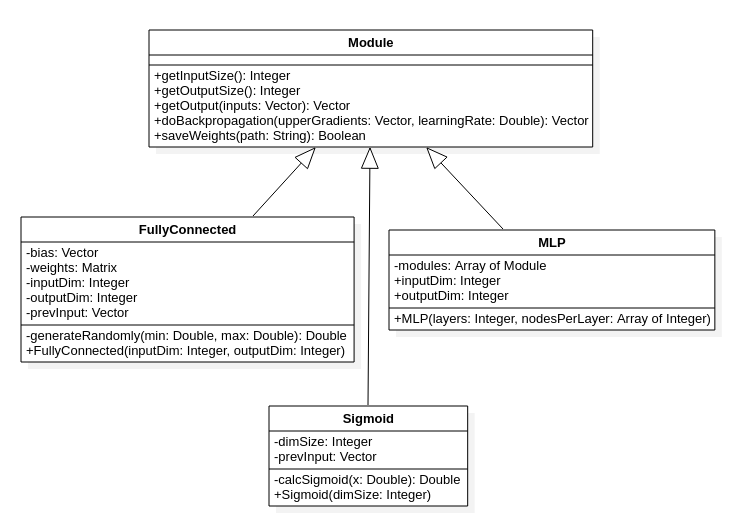
\includegraphics[width=\linewidth]{images/uml-module.png}
		\caption{각 클래스의 관계를 UML로 표현한 그림. Module은 추상 클래스이다.}
		\label{fig:module}
	\end{figure}
	
	\begin{figure}
		\centering
		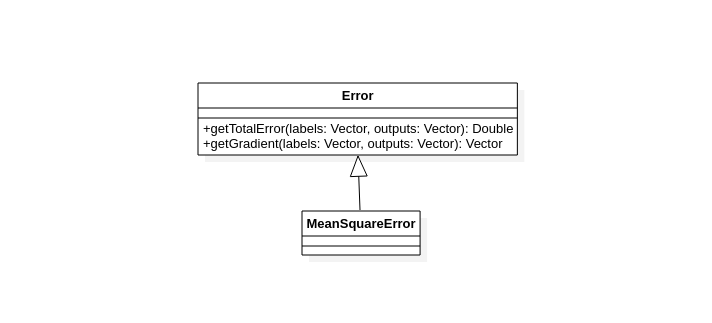
\includegraphics[width=\linewidth]{images/uml-error.png}
		\caption{각 클래스의 관계를 UML로 표현한 그림. Error는 추상 클래스이다.}
		\label{fig:error}
	\end{figure}

	\begin{itemize}
		\item \textbf{FullyConnected}: $n$차원 벡터를 입력으로 받아서 $m$차원 벡터를 출력으로 내는 모듈로, 퍼셉트론에서 입력 벡터에 가중치들을 곱하여 출력 벡터를 만드는 과정과 같다. ($n$과 $m$은 객체의 생성자에서 설정할 수 있다.)
		
		\item \textbf{Sigmoid}: 퍼셉트론을 위해 사용할 수 있는 활성화 함수로, 입력 벡터 $X$의 각 원소 $x_i$에 대하여 아래 식을 적용하여 결과 벡터 $Y$의 각 원소 $y_i$를 계산한다.\\
		\[
		y_i = \sigma (x_i) = \frac{e^{x_i}}{e^{x_i} + 1}
		\]
		그리고 Backpropagation을 수행할 때는 임의의 실수 $x$에 대하여 Sigmoid 함수 $\sigma(x)$의 도함수가 $\sigma'(x)=\sigma(x)(1-\sigma(x))$로 정의된다는 사실에 기반하여, 이전에 들어온 입력 벡터가 $X$일 때 상위 계층에서 전달받은 Gradient에 Sigmoid의 도함수를 곱하여 정의된다.
		
		\item \textbf{MLP}: 본 과제에서 Logic gates와 Donut 데이터를 구분하는 Gate를 학습시키는데 사용된다. 내부적으로 FullyConnected와 Sigmoid를 멤버 변수로 가지고 있고, 입력값에 대한 출력값을 구하는 것은 FullyConnected와 Sigmoid의 getOutput 함수를 순차적으로 호출하는 것으로 구현되고, Backpropagation 역시 역순으로 doBackpropagation 함수를 호출하는 것으로 구현된다.
		
		\item \textbf{MeanSquareError}: 평균 제곱 오차(Mean Square Error)에 따라 실제 정답($y_i$)과 네트워크가 예측한 출력값($\hat{y}_i$)과의 오류값을 계산한다.\\
		\[
		\text{MSE}=\frac{1}{N}\sum_{i=1}^{N} (y_i-\hat{y}_i)^2
		\]
	\end{itemize}

	\subsection{세부 구현 요구 사항 충족 방법}
	
	본 과제의 명세서에는 다음과 같은 구현 요구 사항이 명시되어있다.
	
	\begin{enumerate}
		\item Layer 수, Layer 당 node 수는 변수로 지정할 것.
		\item 한 층 계산이 하나의 함수가 되도록 구현.
		\item weight는 행렬 형식으로 파일에 저장.
	\end{enumerate}

	아래 Section은 각 요구 사항을 코드 상에서 어떻게 구현하였는지를 간단하게 설명한 것이다.
	
	\subsubsection{Layer 수, Layer 당 node 수는 변수로 지정할 것}
	
	MLP에 존재하는 Fully Connected Layer의 수, 각 Layer에 존재하는 Node의 수를 MLP 객체를 생성할 때 결정할 수 있도록 MLP의 생성자를 작성하였다. 구현한 MLP의 생성자는 아래와 같은 선언을 가지고 있다.
	
	\verb|MLP(const int layers, const int nodesPerLayer[]);|
	
	첫 번째 매개변수 \verb|layers|는 입력층, 은닉층, 출력층 모두를 포함한 전체 레이어의 개수를 의미하고, 두 번째 매개변수 \verb|nodesPerLayer[]|는 각 레이어에 존재하는 Node의 수를 저장한 배열이다. (이 배열의 길이는 \verb|layers|와 같아야 하며, 각 노드의 활성화 함수는 Sigmoid이다.)
	
	이 생성자의 매개변수를 조절함으로써 다양한 MLP를 생성할 수 있는데 예를 들어, Logic Gate를 Simulate 하기 위한 Single-Layer Perceptron은 \verb|MLP(2, { 2, 1 })|와 같이, Node가 3개 존재하는 은닉층 한 개를 가진 MLP는 \verb|MLP(3, { 2, 2, 1 })|과 같이 생성할 수 있다.
	
	\subsubsection{한 층 계산이 하나의 함수가 되도록 구현}
	
	한 MLP 전체의 출력값을 계산하는 것은 MLP 객체의 \verb|getOutput| 함수에서 이루어지는데, 이 함수 내부에서 각 층의 출력값을 각 Module의 \verb|getOutput| 함수로 계산한다. 즉, 한 층의 출력값을 계산하는 것이 하나의 함수 \verb|getOutput|가 되도록 구현되었다.
	
	\subsubsection{weight는 행렬 형식으로 파일에 저장}
	
	\verb|main|함수에서 Logic gate와 Donut 구분 MLP를 학습시키고 난 뒤 MLP에 존재하는 모든 Fully Connected Layer의 Weight 행렬을 \verb|result| 디렉토리에 저장한다. 이는 MLP 객체의 \verb|saveWeights| 함수를 호출하는 방식으로 구현되며, MLP 내부에서는 각 Module의 \verb|saveWeights| 함수를 재귀적으로 호출한다.
	
	\subsection{소스 파일 구조}
	
	본 과제의 C++ 퍼셉트론 코드는 총 6개의 소스 파일로 구성된다.
	
	\begin{itemize}
		\item \textbf{Modules.h, Modules.cpp}: MLP를 구현하는데 필요한 각 모듈들을 클래스로 정의한다.
		\item \textbf{MLP.h, MLP.cpp}: Modules.h에서 정의한 모듈을 이용하여 Multi-Layer Perceptron을 구현한다. 출력값을 구하는 과정과 역전파를 하는 과정 모두 각 모듈의 멤버 함수를 호출하는 것으로 구현된다.
		\item \textbf{Main.cpp}: AND, OR, XOR logic gate와 Donut data를 구분하는 모델을 MLP 클래스를 이용하여 학습시키고, 학습 후 결과(모든 가중치 행렬, 각 에폭 당 Error 값)를 CSV 파일로 저장한다. 추후 이 CSV 파일을 이용하여 학습 결과를 시각적으로 보여주는 그래프를 그린다.
		\item \textbf{Main.out}: 2.1에서 설명하는 실행 환경에서 빌드한 실행 파일이다.
		\item \textbf{Makefile}: 소스 빌드 방법을 정의한 Makefile로, build-essential 패키지가 설치된 Linux 환경에서 ’make’ 명령어를 이용하여 빌드할 수 있다.
	\end{itemize}
	
	\section{실행 결과}
	
	\subsection{퍼셉트론 실행 환경}
	
	본 과제의 소스 코드는 Ubuntu 20.04 LTS (x86) 에서 개발 및 테스트 되었다. 순차적인 빌드 및 실행 방법은 아래와 같다.
	
	\begin{enumerate}
		\item Ubuntu 20.04 LTS와 같은 리눅스 환경에서 GCC를 이용하여 C++을 컴파일하기 위해 build-essential 패키지를 설치한다. (sudo apt install build-essential)
		\item 본 보고서와 함께 첨부된 소스 폴더(Makefile이 존재하는 디렉토리)에서 터미널을 실행하고, `make` 명령어를 실행한다.
		\item 빌드 결과 생성된 Main.out 파일을 실행한다.
		\item 프로그램이 종료되면 해당 디렉토리에 \verb|results|라는 새로운 디렉토리가 생성되고, 그 디렉토리 내에 모든 결과 데이터가 저장된다.
	\end{enumerate}
	
	\subsection{퍼셉트론 실행 결과}
	
	위에서 설명한 실행 방법에 따라 퍼셉트론 학습 프로그램을 실행할 경우 아래와 같은 출력이 나타난다. 매 실행마다 랜덤 시드 값이 재설정되므로 정확한 출력은 다를 수 있으며, 경우에 따라 XOR 게이트는 올바르게 학습되지 않는 경우도 발생할 수 있다. Iteration은 최대 $500,000$회 진행될 수 있고, 그 이전에 MSE의 평균값이 $10^{-3}$보다 작아질 경우 조기 종료된다.
	
	그리고 프로그램이 완료되면 \textbf{results}라는 이름의 서브 디렉토리에 학습 결과가 저장된다. (CSV 형식)
	
	\begin{minted}
		[
		frame=lines,
		framesep=2mm,
		baselinestretch=1.2,
		fontsize=\footnotesize,
		linenos
		]
		{text}
Training AND Gate...
	Successfully trained AND Gate! (after 24566 iterations)
	Saved weight matrices. (./results/AND)
	Saved error history. (./results/AND/error.csv)
Training OR Gate...
	Successfully trained OR Gate! (after 13205 iterations)
	Saved weight matrices. (./results/OR)
	Saved error history. (./results/OR/error.csv)
Training XOR Gate...
	Successfully trained XOR Gate! (after 47945 iterations)
	Saved weight matrices. (./results/XOR)
	Saved error history. (./results/XOR/error.csv)
Training Donut Gate...
	Successfully trained Donut Gate! (after 189699 iterations)
	Saved weight matrices. (./results/Donut)
	Saved error history. (./results/Donut/error.csv)
	\end{minted}
	
	\subsection{그래프 시각화}
	
	아래의 Figure 3, 4가 학습 결과를 그래프로 그린 결과이다. (plot-error.py, plot-seperators.py)
	
	결과적으로 각 Gate의 Error는 모두 0으로 수렴하였고, MLP의 첫번째 은닉층의 가중치 행렬을 이용하여 직선 그래프를 그리면 각 직선 그래프가 정답이 0인 정점과 1인 정점을 가르도록 학습되었다는 것을 알 수 있다.
	
	\begin{figure}
		\centering
		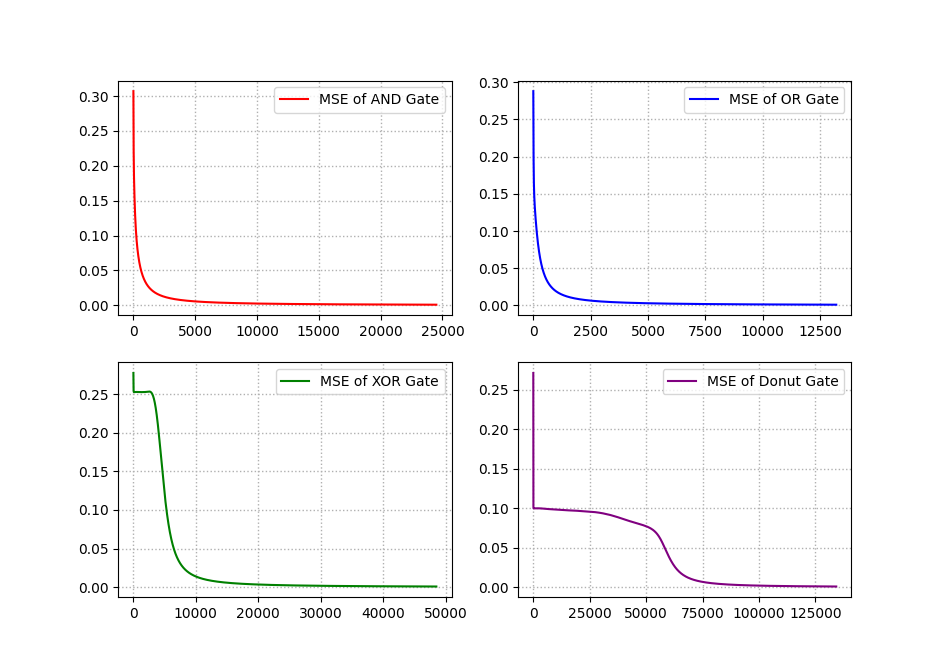
\includegraphics[width=\linewidth]{images/graph-error.png}
		\caption{각 MLP의 iteration 당 MSE 값을 나타낸 것이다. 결과적으로 모두 0에 수렴하였다.}
	\end{figure}
	
	\begin{figure}
		\centering
		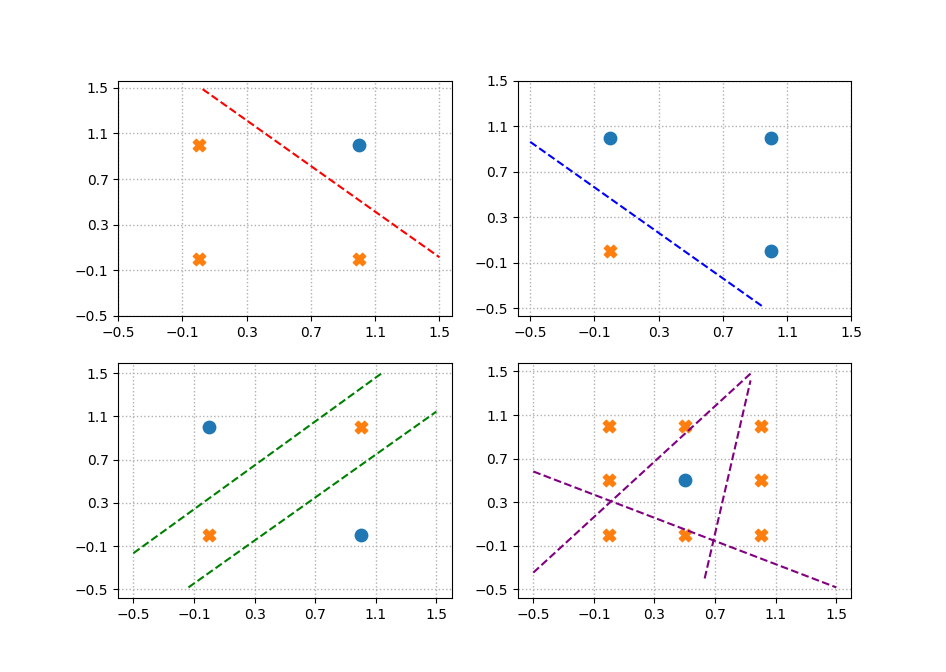
\includegraphics[width=\linewidth]{images/graph-lines.png}
		\caption{각 MLP의 첫 번째 은닉층의 가중치 행렬을 이용하여 기준 선을 그린 그림이다.}
	\end{figure}
	
\end{document}
